\section{Deployment}

In this section, we'll cover the deployment process for your email marketing tool. We'll discuss setting up CI/CD pipelines, deploying backend services and the front-end deployment.

\subsection{Deployment Process}

\begin{enumerate}
    \item \textbf{CI/CD Pipeline Creation:}
        \begin{itemize}
            \item Set up a CI/CD pipeline using GitLab CI/CD.
            \item Configure pipeline stages for building, deployment and database schema migration.
        \end{itemize}
    
    \item \textbf{Backend Deployment:}
        \begin{itemize}
            \item Containerize backend services using Docker.
            \item Create Dockerfiles for the email service.
            \item Define a `docker-compose.yml` file for managing the email service and database containers.
            \item Deploy backend containers to a Azure.
        \end{itemize}
    
    \item \textbf{Front-End Deployment:}
        \begin{itemize}
            \item Deploy the Vue.js front-end application separately.
            \item Use Vercel for front-end deployment.
            \item Configure Vercel project settings environment variables.
        \end{itemize}
\end{enumerate}

\clearpage
\subsection{Deployment Diagram}

Figure \ref{fig:Sprint 3 Deployment Diagram} illustrates the deployment of our app.


\begin{figure}[ht]
	\centering
	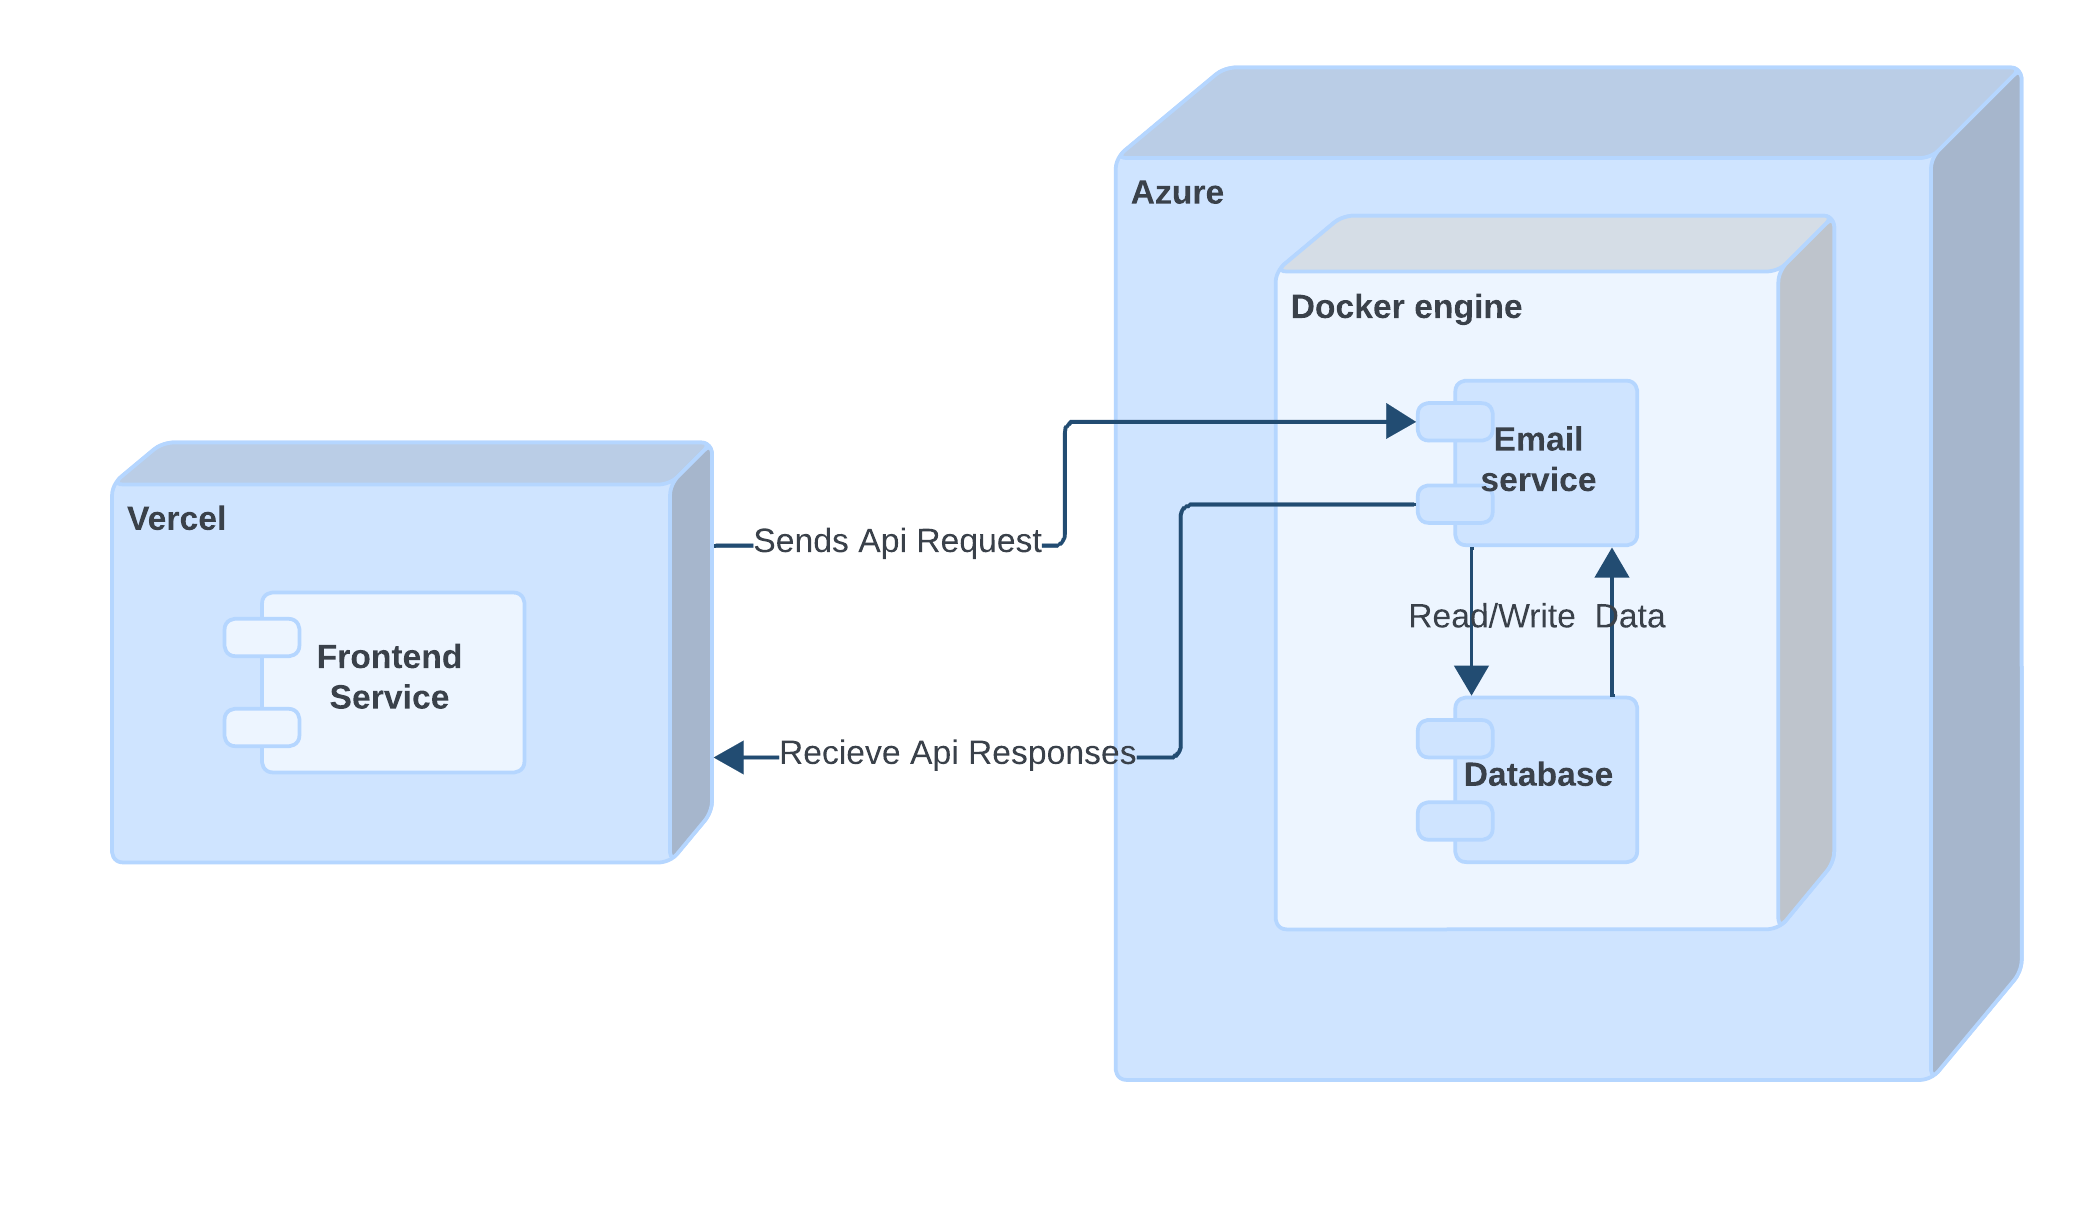
\includegraphics[width=0.7\linewidth]{Images/Sprint3/deployment diagram v2.png}
	\caption{ Deployment Diagram}
	\label{fig:Sprint 3 Deployment Diagram}
\end{figure}

\subsection{CI/CD Pipeline Diagram}

Figure \ref{fig:Sprint 3 CI/CD Pipeline Diagram} illustrates the stages of the CI/CD pipline.

\begin{figure}[ht]
	\centering
	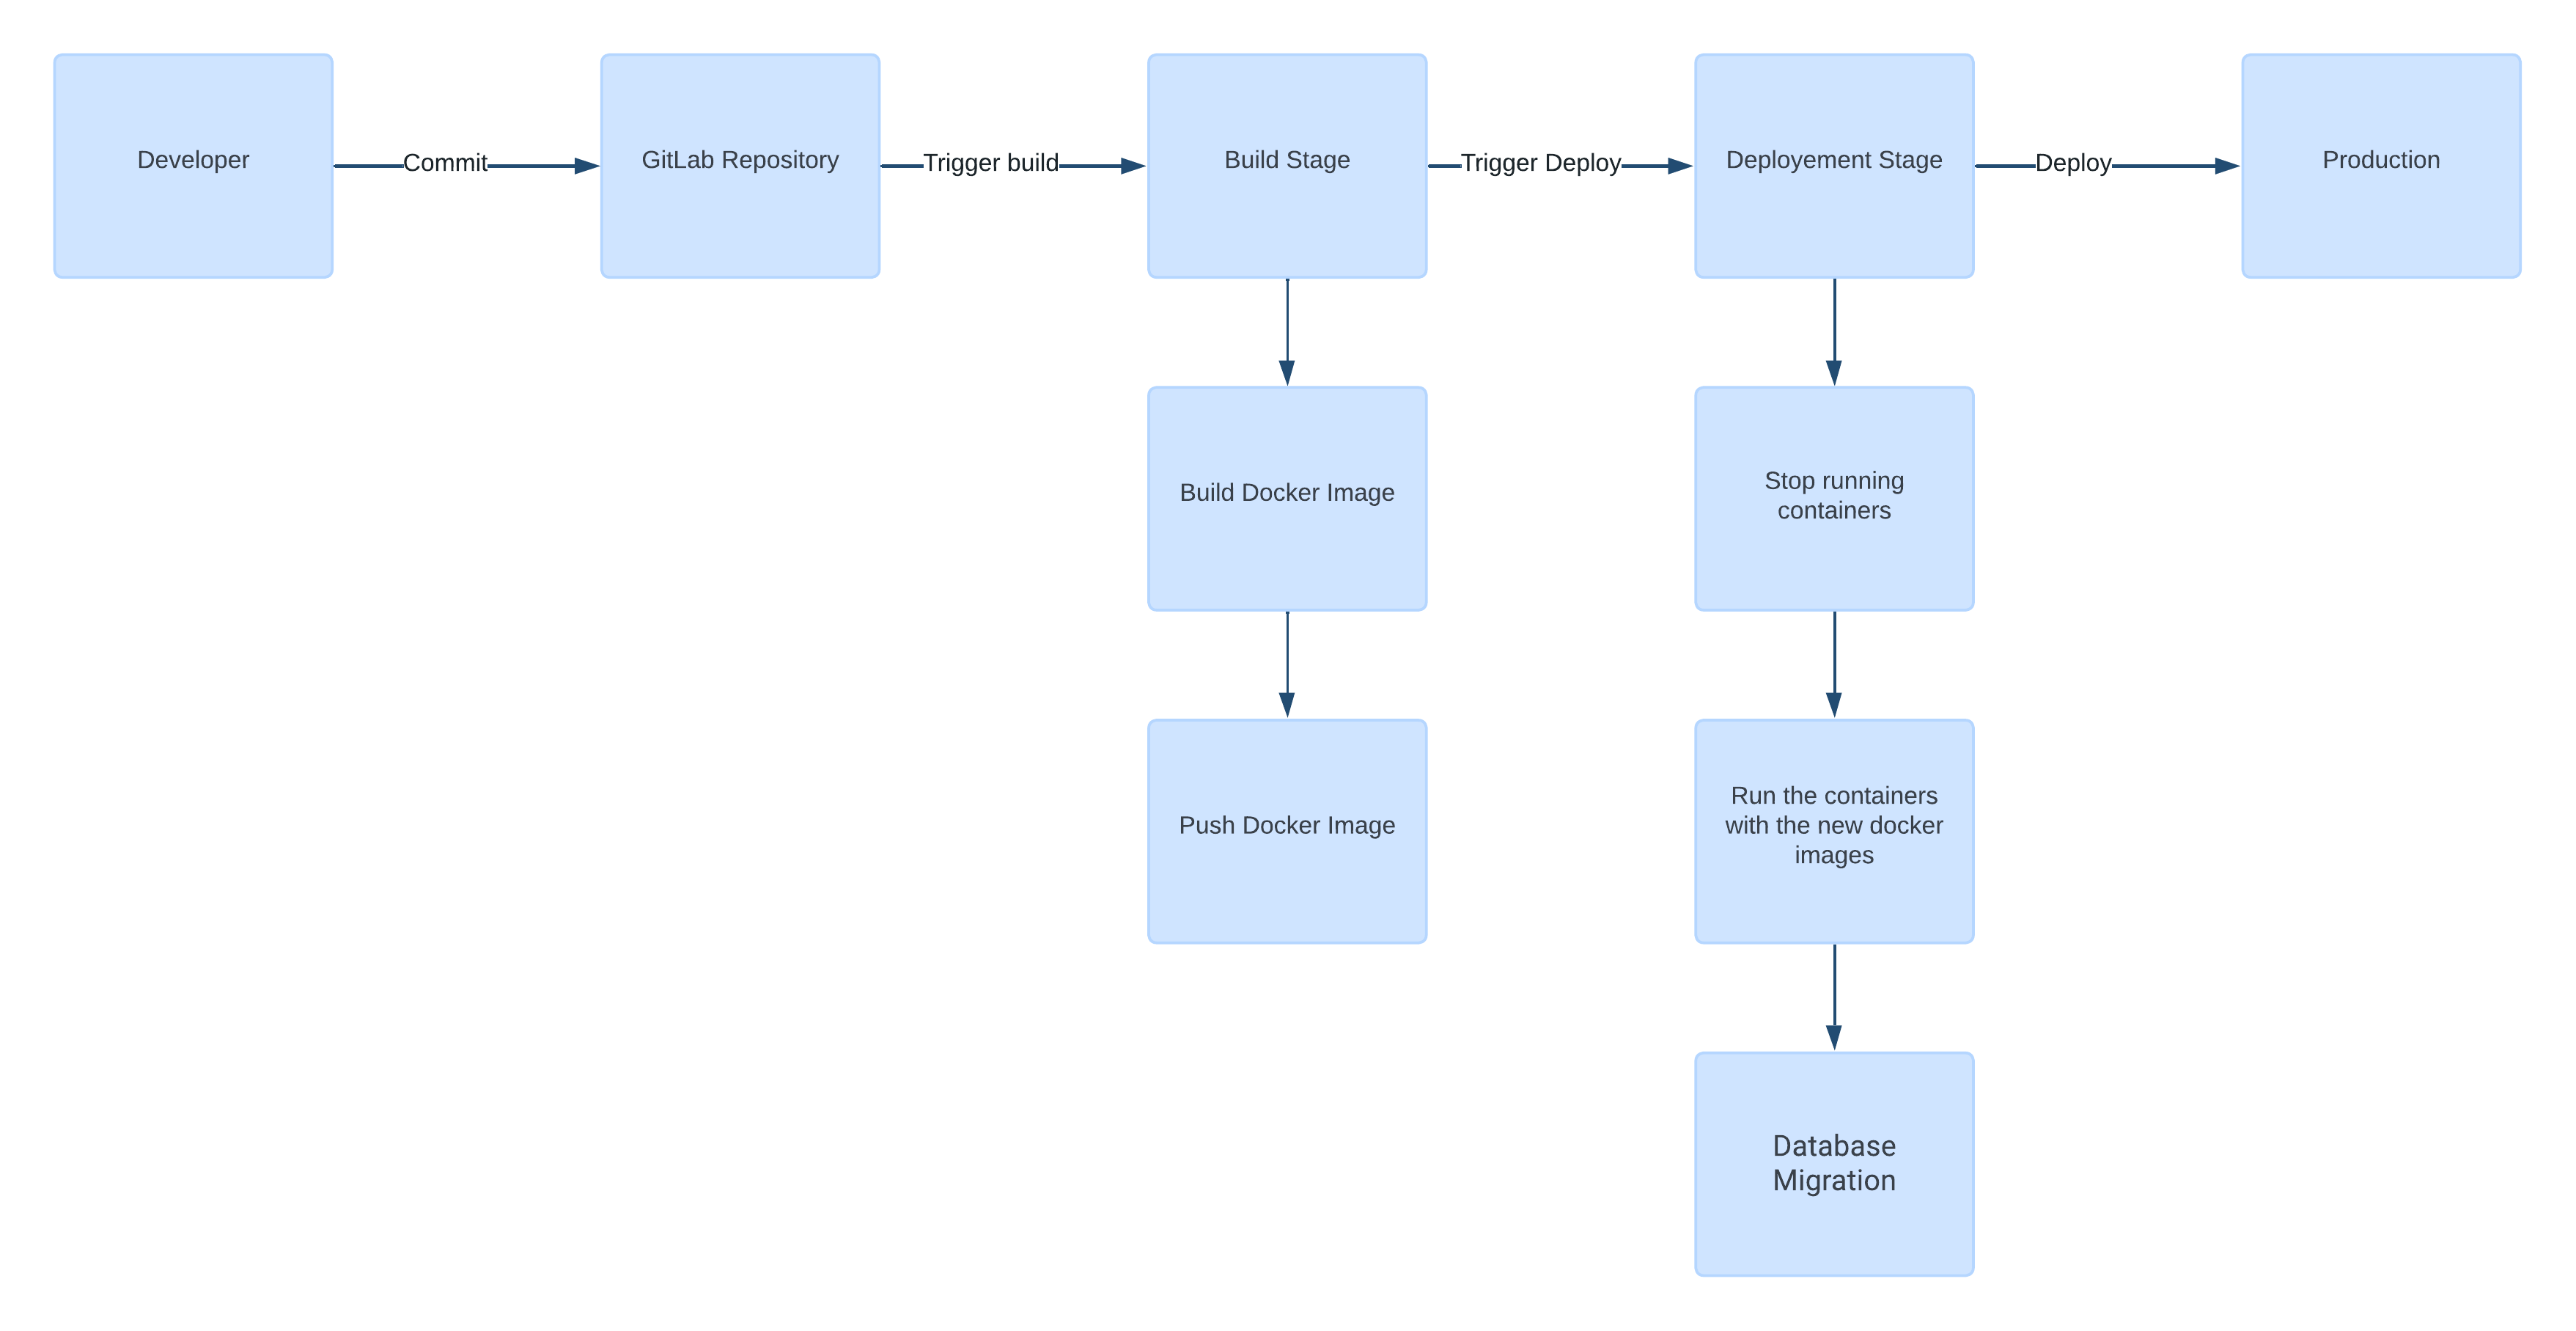
\includegraphics[width=0.7\linewidth]{Images/Sprint3/ci_pipline_diag.png}
	\caption{ CI/CD Pipeline Diagram}
	\label{fig:Sprint 3 CI/CD Pipeline Diagram}
\end{figure}
